\documentclass[11pt]{article}
\usepackage[a4paper, margin=2.2cm]{geometry}
\usepackage{amsmath, amssymb, amsthm}
\usepackage{graphicx}
\usepackage{booktabs}
\usepackage{xcolor}
\usepackage{hyperref}
\usepackage[T1]{fontenc}
\usepackage{listings}
\hypersetup{colorlinks=true, urlcolor=blue!60!black, linkcolor=blue!60!black}

\title{Butane dihedral barrier crossing in water:\\
       reactive flux vs.\ memory kernel + anharmonicity}
\author{David Girardier --- working note}
\date{\today}

\newcommand{\rad}{\mathrm{rad}}
\newcommand{\ps}{\mathrm{ps}}
\newcommand{\fs}{\mathrm{fs}}
\newcommand{\GH}{\mathrm{GH}}
\newcommand{\RF}{\mathrm{RF}}
\newcommand{\GLE}{\mathrm{GLE}}

\begin{document}
\maketitle

\section{Question}

The Grote--Hynes (GH) transmission coefficient $\kappa_\GH$ is computed
from the extracted memory kernel $K(t)$ via the implicit equation
\begin{equation}
\lambda_r = \frac{\omega_b^2}{\lambda_r + \widehat{K}(\lambda_r)},
\qquad
\kappa_\GH = \lambda_r/\omega_b,
\label{eq:gh}
\end{equation}
which assumes a \emph{parabolic} barrier of curvature $\omega_b^2$.
For butane dihedral in water, kernel-based GH gives $\kappa_\GH \approx 0.89$,
yet the direct reactive-flux measurement gives $\kappa_\RF \approx 0.25$
--- a factor of $\sim$3.5 disagreement. We test the hypothesis that the
gap is due to \emph{anharmonicity} of the dihedral PMF away from $\phi_b$
(rather than a kernel-extraction problem) by running a 1D generalized
Langevin equation (GLE) with the same extracted $K(t)$ and the
\emph{full} mean-force spline, and measuring its reactive flux directly.

\section{System and shooting protocol}

GROMOS 53A6 united-atom butane in 722 SPC/E waters
(GROMACS~2020.7 with PLUMED~2.9 for the dihedral CV). NPT, $T = 300$\,K,
$P = 1$\,atm, all-angle constraints. Reaction coordinate is the dihedral
$\phi$. Working with the \emph{eclipsed} barrier at
$\phi_b \approx 120^\circ$ (PLUMED) $\equiv 245^\circ$ (numpy convention),
between the trans and gauche$^+$ wells.

\paragraph{Phase A --- bath equilibration.}
Single 1500\,ps trajectory with PLUMED \texttt{RESTRAINT KAPPA=10000} at
$\phi_b$, warm-up 500\,ps, then 51 bath snapshots saved every 20\,ps
($\rightarrow$ \texttt{shooting\_barrier/equil/config\_*.gro}).

\paragraph{Phase B --- shooting.}
For each seed $i = 1\dots N_\mathrm{shoot}$, free dynamics of 10\,ps
(5001 frames at $\Delta t = 2\,\fs$), \texttt{gen-vel=yes,
gen-seed=$i$}, no PLUMED restraint. Each seed picks one of the 51 bath
configs cyclically. Recorded per frame: $\phi(t)$, $J\!\cdot\!v$
(generalized velocity through the dihedral Jacobian), and
$\ddot\phi$ via central FD. Saved as
\texttt{shoot\_seed\{i\}/phi\_data.npz}.
Currently $N = 1006$ trajectories with valid \texttt{phi\_data.npz}
(seed 807 orphaned: TRR present, post-processing interrupted). Of these,
$N_\mathrm{accept} = 663$ have $|\phi(0) - \phi_b| < 10^\circ$ and are
used as ``barrier-top'' trajectories.

\paragraph{Code.} \texttt{gromacs\_run/shooting\_barrier/run\_shooting\_barrier.py}.

\section{Kernel extraction}

Two extractors are available, both starting from the cold-start
out-of-equilibrium least-squares formulation
(\texttt{kernel\_extraction/nonstationary\_kernel\_lsq.py}):
\begin{description}
\item[Free-LSQ:] \texttt{extract\_kernel\_lsq} returns the kernel sampled
on the discrete time grid $\Delta t_e = 5 \Delta t = 10\,\fs$ as a free
$n$-vector. Tikhonov-smoothness regularized; here truncated to $500\,\fs$.
\item[Prony NLSQ:] \texttt{extract\_kernel\_prony} parameterises
$K(t) = \sum_{k=1}^{n_\mathrm{exp}} a_k \exp(-t/\tau_k)$ and fits
$(a_k, \tau_k)$ by nonlinear least squares against the same Toeplitz
system. We added a \texttt{tau\_bounds=$(\tau_\mathrm{min},
\tau_\mathrm{max})$} option to prevent runaway slow tails at large $N$.
\end{description}
Both use the binned mean force $\langle\ddot\phi\,|\,\phi\rangle$ as the
deterministic part. The barrier curvature
$\omega_b = \sqrt{|U''(\phi_b)|} = 24.29\,\rad/\ps$ is read from the
spline second derivative at $\phi_b$.

\section{GLE simulation of $\kappa(t)$}

For a given $K(t)$ and mean force $F(\phi)$, the GLE
\begin{equation}
\ddot{\phi}(t) = F(\phi(t))
- \int_0^t K(t-s)\,\dot\phi(s)\,ds + \eta(t),
\qquad
\langle \eta(t)\eta(t') \rangle = \beta_\mathrm{eff} K(|t-t'|),
\end{equation}
is integrated numerically. Two integrators are implemented in
\texttt{kernel\_extraction/benchmark\_extended\_cases.py}:
\begin{enumerate}
\item \texttt{generate\_gle\_multiexp}: one Mori auxiliary variable per
exponential of a Prony kernel. OU noise with FDT, exact in continuous
time; numerically explicit (Euler--Maruyama) on the auxiliaries.
\item \texttt{generate\_gle\_arbitrary}: arbitrary numeric $K(t)$.
Friction term computed as $\Delta t \sum_j K_j v_{i-j}$
(rectangle convolution). Colored noise via spectral filter:
$\eta = \mathrm{IFFT}\bigl(\sqrt{\Re\widetilde{C}}\;
\mathrm{FFT}(w)\bigr)$ where $w$ is unit-variance white noise and
$\widetilde{C} = \mathrm{FFT}(\beta_\mathrm{eff} K)$ is the discrete
spectral density of the autocovariance. The
$\sqrt{S}$ scaling (without the spurious $\Delta t$ factor present in
the original code) reproduces $\langle \eta_i \eta_j \rangle =
\beta_\mathrm{eff}\, K(|i-j|\,\Delta t)$ exactly for circulant
covariances.
\end{enumerate}
The effective inverse temperature is read from the data:
$\beta_\mathrm{eff} = \langle \dot\phi(0)^2 \rangle = 30.29\,\rad^2/\ps^2$.
Initial conditions: $\phi(0) = \phi_b$, $\dot\phi(0) \sim
\mathcal{N}(0,\sqrt{\beta_\mathrm{eff}})$, auxiliaries from their
stationary distribution.

The reactive flux estimator
\begin{equation}
\kappa(t) = \frac{2\,\langle \dot\phi(0)\,
\theta(\phi(t) - \phi_b)\rangle}{\langle |\dot\phi(0)| \rangle}
\end{equation}
is then computed both from the MD shoots (gives $\kappa_\RF$) and from
the GLE shoots (gives $\kappa_\GLE$). For the GLE the run is
$T = 5\,\ps$, $\Delta t_\mathrm{GLE} = 1\,\fs$, $N_\mathrm{traj} = 5000$.

\section{Results}

\subsection{Headline numbers (N = 663, nbins=36, polyfit $\omega_b$)}

\begin{center}
\begin{tabular}{lccc}
\toprule
Method & $\kappa$ plateau & Comment \\
\midrule
$\kappa_\RF$ (MD shoots)             & $\mathbf{0.250}$       & reactive flux, 3--8\,ps plateau \\
$\kappa_\GH$ (Free-LSQ kernel)        & $0.899$                 & analytic, eq.~(\ref{eq:gh}) \\
$\kappa_\GLE^{\,\mathrm{harm}}$       & $0.889$                 & parabolic $F$, sanity check \\
$\kappa_\GLE^{\,\mathrm{anharm}}$     & $\mathbf{0.241/0.223}$  & full $F(\phi)$ spline (stride=5\,/\,1) \\
\bottomrule
\end{tabular}
\end{center}
The harmonic-barrier GLE reproduces the analytic $\kappa_\GH$ within
1\,\%, validating the integrator and FDT noise scaling. Replacing the
parabolic $F$ with the full anharmonic spline drops $\kappa$ from 0.90
to ${\sim}0.23$ --- recovering $\kappa_\RF = 0.25$ within $\sim$5--10\,\%.
The two anharmonic values bracket the result depending on the kernel
sampling stride: stride=5 ($\Delta t_e = 10\,\fs$) is the value used
throughout the convergence figure (Fig.~\ref{fig:conv}); stride=1
($\Delta t_e = 2\,\fs$) gives a slightly lower $K(0)$ and a slightly
more dissipative effective kernel.

\paragraph{$\omega_b$ extraction.}
The barrier curvature is obtained by a parabolic polyfit of the
free-energy profile (from cumulative integration of the binned
$\langle\ddot\phi\,|\,\phi\rangle$) on a narrow window
$|\phi - \phi_b| < 0.15\,\rad$, giving $\omega_b = 24.2\,\rad/\ps$.
This polyfit estimate is stable to the bin choice (24.0--24.5 for
nbins\,$\in\{24,36,48\}$, only the 60-bin case dips to 20.6 from a
local PMF artifact). The naive second-derivative-of-the-spline at
$\phi_b$ is much less robust: it varies from 3.3 to 25.9 across the
same range of bin counts, and was the source of an earlier inflation
of $\kappa_\GH$.

\paragraph{Stride sensitivity.}
Subsampling the trajectories before the kernel extraction (stride 1, 2,
5, 10 corresponding to $\Delta t_e = 2,\,4,\,10,\,20\,\fs$) shifts
$K(0)$ by up to 25\,\% but the integrated friction $\gamma_\mathrm{int}
= \int K\,dt$ only by $\sim 8\,\%$. Consequently $\kappa_\GLE$ moves by
no more than $\pm 0.04$ across this range, which is within the
$\kappa_\GLE/\kappa_\RF$ scatter at $N=663$.

\paragraph{$\phi(0)$ centering.}
The 663 accepted barrier-top trajectories have
$\phi(0) = 244.99^\circ$ (target $\phi_b = 245.00^\circ$),
$\sigma_{\phi(0)} = 3.14^\circ$, range $[236.3, 250.2]^\circ$ ---
i.e.\ the shoots are tightly localised at the barrier, so any visual
parabola misfit in earlier figures is a curvature-extraction issue,
not a shooting-protocol issue.

\subsection{Convergence with sample size}

The script \texttt{butane\_kappa\_convergence.py} repeats the comparison
on bootstrap subsamples $N \in \{50, 100, 150, 200, 300, 500, 663\}$,
recomputing $\kappa_\RF$ on the same subsample as the kernel fit.
Both estimators converge to the same plateau as $N$ grows; at
$N \sim 100$ they already agree to within ${\sim}10$\,\% but each is
still noisy on its own. The full $N = 663$ result is reliable.
See Fig.~\ref{fig:conv}.

\begin{figure}[h]
\centering
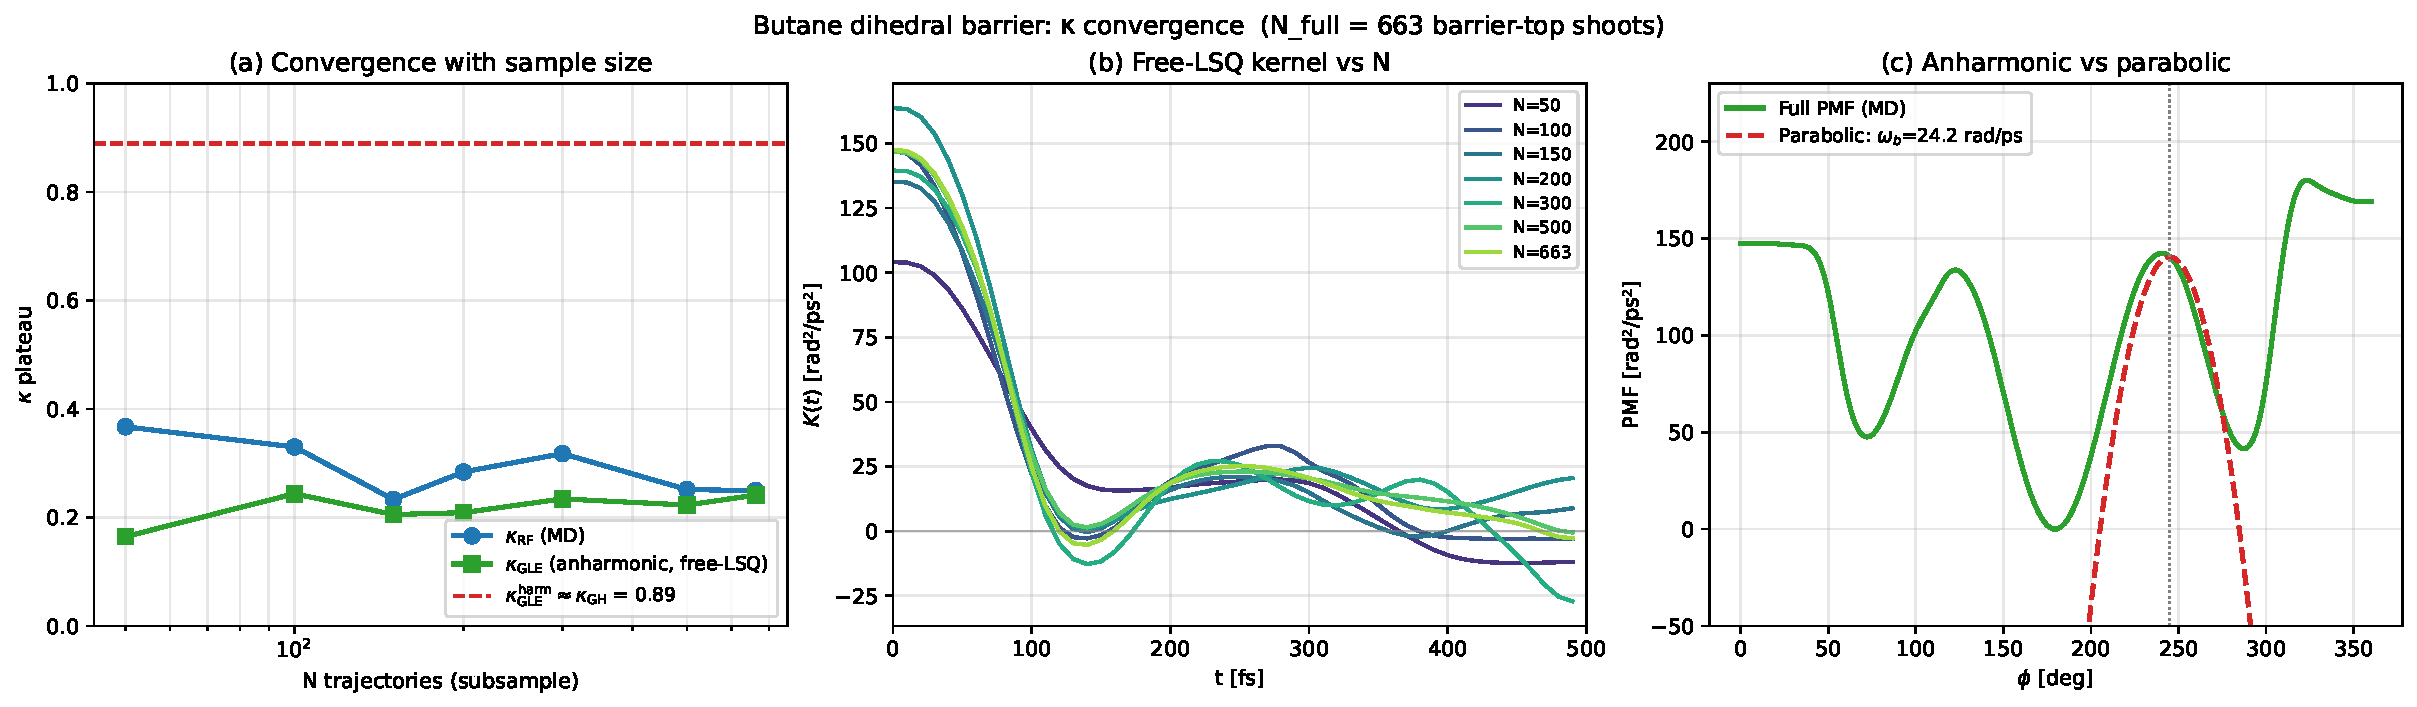
\includegraphics[width=\linewidth]{butane_kappa_convergence.pdf}
\caption{(a) $\kappa_\RF$ (MD) and $\kappa_\GLE^{\,\mathrm{anharm}}$
(GLE with full mean force) as functions of the sample size $N$ used
for both estimators. The dashed line shows
$\kappa_\GLE^{\,\mathrm{harm}} \approx \kappa_\GH$ at full $N$.
(b) Free-LSQ kernel for the same subsamples.
(c) Full PMF (from binned $\langle\ddot\phi\,|\,\phi\rangle$) compared
to the parabolic approximation at $\phi_b$.}
\label{fig:conv}
\end{figure}

\subsection{Why Prony alone is misleading}

A 2-exponential Prony fit on the full $N = 663$ dataset returns one
fast component $(a, \tau) \approx (248,\,40\,\fs)$ matching the
1-exponential fit, plus a \emph{second} slow component
$(13,\,10\,\ps)$ whose integrated friction (130\,$\rad/\ps$) is an
order of magnitude larger than the fast one but contributes negligibly
to $\widehat{K}(\lambda_r)$ at the GH solution
($\lambda_r \approx 6\,\rad/\ps$). It is, however, dynamically active
in the GLE simulation, where it depresses $\kappa_\GLE$ to $\approx 0.32$
instead of $0.24$. Switching to the Free-LSQ numeric kernel (truncated
at $500\,\fs$) avoids this artifact entirely.

\section{Code map}

\begin{lstlisting}[basicstyle=\ttfamily\footnotesize, breaklines=true]
gromacs_run/shooting_barrier/
   run_shooting_barrier.py    # GROMACS shooting from phi_b ~ 120 deg
   equil/                      # 51 bath configs
   shoot_seed{1..1007}/        # phi_data.npz per seed (1006 valid)
testASE/butane_dihedral_water/
   butane_rf_vs_kernel.py      # RF vs kernel-derived GH kappa; t0 sweep
   butane_gle_kappa.py         # GLE kappa simulation:
                               #   --method {prony2|free-lsq}
                               #   --n-traj-fit N
                               #   --lsq-trunc-fs 500
   butane_kappa_convergence.py # kappa vs N subsample
   butane_gle_overleaf.tex     # this document
kernel_extraction/
   nonstationary_kernel_lsq.py # Free-LSQ extractor
   benchmark_prony_nlsq.py     # Prony NLSQ extractor (tau_bounds option)
   benchmark_extended_cases.py # GLE integrators (multi-exp + arbitrary)
\end{lstlisting}

\section{Open questions}
\begin{itemize}
\item Compare the LSQ kernel against the equilibrium VolterraBasis kernel
from the 40\,ns unbiased run (plan 4, step 3).
\item Position-dependent kernel $K(\phi_0, t)$: existing
\texttt{PositionalKernel\_fd.py} extracts $K(\phi, t)$ from the same
shoots; not yet inserted into the GLE.
\item Repeat the protocol from the trans well (plan 2--4) and check the
implied gauche$\leftrightarrow$trans rate against Eyring/Kramers.
\item Decide whether the residual $0.241 \to 0.250$ gap is statistical
(\,$\sigma$ on $\kappa_\GLE$ from $N_\mathrm{traj} = 5000$\,) or due to
multidimensional reaction-coordinate effects.
\end{itemize}

\end{document}
